\documentclass[10pt]{article}
\usepackage[utf8]{inputenc}
\usepackage[T1]{fontenc}
\usepackage{amsmath}
\usepackage{amsfonts}
\usepackage{amssymb}
\usepackage[version=4]{mhchem}
\usepackage{stmaryrd}
\usepackage{bbold}
\usepackage{graphicx}
\usepackage[export]{adjustbox}
\graphicspath{ {./images/} }
\usepackage{hyperref}
\hypersetup{colorlinks=true, linkcolor=blue, filecolor=magenta, urlcolor=cyan,}
\urlstyle{same}

\title{Text Representation Learning }

\author{}
\date{}


\begin{document}
\maketitle
Machine Learning Course - CS-433

Dec 6, 2023

Martin Jaggi

Last updated on: December 3, 2023

$$
\square
$$

\section*{Motivation}
Finding numerical representations for words is fundamental for all machine learning methods dealing with text data.

Goal: For each word, find mapping (embedding)

$$
w_{i} \mapsto \mathbf{w}_{i} \in \mathbb{R}^{K}
$$

Representation should capture semantics of the word.

\begin{center}
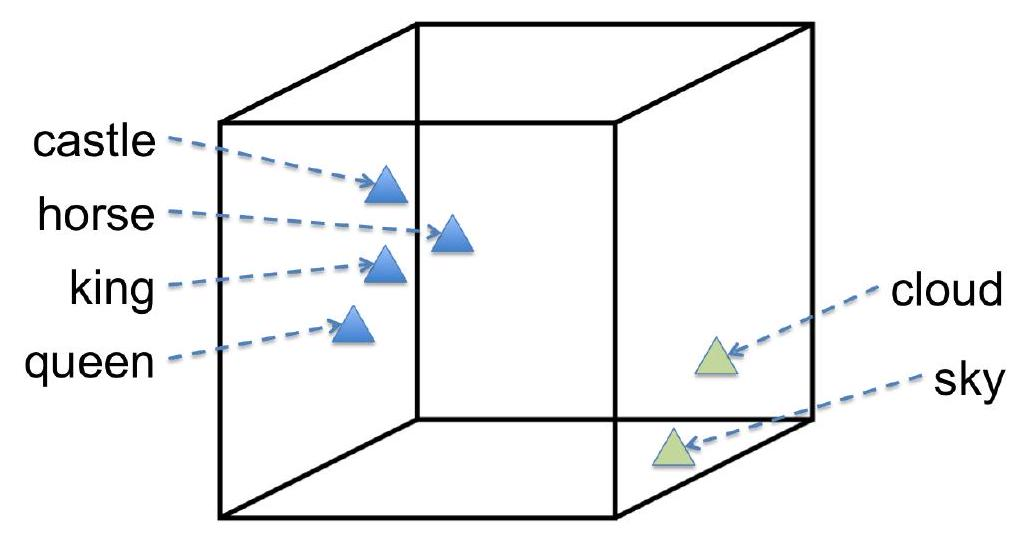
\includegraphics[max width=\textwidth]{2023_12_29_a68c38042b8470fb184bg-02}
\end{center}

Constructing good feature representations ( $=$ representation learning) benefits all ML applications.

\section*{The Co-Occurence Matrix}
A big corpus of un-labeled text can be represented as the co-occurrence counts

$n_{i j}:=$ \#contexts where word $w_{i}$ occurs together with word $w_{j}$.

\begin{center}
\begin{tabular}{|l|l|l|l|l|}
\hline
 & 1 & 1 &  &  \\
\hline
 &  & 3 &  &  \\
\hline
 & 1 &  &  &  \\
\hline
 & 2 &  & 1 &  \\
\hline
1 &  &  &  & 1 \\
\hline
 &  & 1 &  &  \\
\hline
 & 1 &  & 1 & 1 \\
\hline
\end{tabular}
\end{center}

Needs definition of

\begin{itemize}
  \item Context e.g. document, paragraph, sentence, window
  \item Vocabulary
\end{itemize}

$$
\mathcal{V}:=\left\{w_{1}, \ldots, w_{D}\right\}
$$

For words $w_{d}=1,2, \ldots, D$ and context words $w_{n}=1,2, \ldots, N$, the co-occurence counts $n_{i j}$ form a very sparse $D \times N$ matrix.

\section*{Learning Word-Representations (Using Matrix Factorization)}
Find a factorization of the cooccurence matrix!

Typically uses $\log$ of the actual counts, i.e. $x_{d n}:=\log \left(n_{d n}\right)$.

We will aim to find $\mathbf{W}, \mathbf{Z}$ s.t.

$$
\mathbf{X} \approx \mathbf{W} \mathbf{Z}^{\top}
$$

So for each pair of words $\left(w_{d}, w_{n}\right)$, we try to 'explain' their co-occurence count by a numerical representation of the two words

\begin{itemize}
  \item in fact by the inner product of the two feature vectors $\mathbf{W}_{d:}, \mathbf{Z}_{n:}$.
\end{itemize}

$$
\min _{\mathbf{W}, \mathbf{Z}} \mathcal{L}(\mathbf{W}, \mathbf{Z}):=\frac{1}{2} \sum_{(d, n) \in \Omega} f_{d n}\left[x_{d n}-\left(\mathbf{W} \mathbf{Z}^{\top}\right) d n\right]^{2}
$$

where $\mathbf{W} \in \mathbb{R}^{D \times K}$ and $\mathbf{Z} \in \mathbb{R}^{N \times K}$ are tall matrices, having only $K \ll$ $D, N$ columns.

The set $\Omega \subseteq[D] \times[N]$ collects the indices of non-zeros of the count matrix $\mathbf{X}$.

Each row of those matrices forms a representation of a word $(\mathbf{W})$ or a context word $(\mathbf{Z})$ respectively.

\section*{GloVe}
This model is called GloVe, and is a variant of word2vec.

Weights $f_{d n}$ : Give "importance" of each entry. Choosing $f_{d n}:=1$ is ok. GloVe weight function:

$f_{d n}:=\min \left\{1,\left(n_{d n} / n_{\max }\right)^{\alpha}\right\}, \quad \alpha \in[0 ; 1] \quad$ e.g. $\alpha=\frac{3}{4}$

\begin{center}
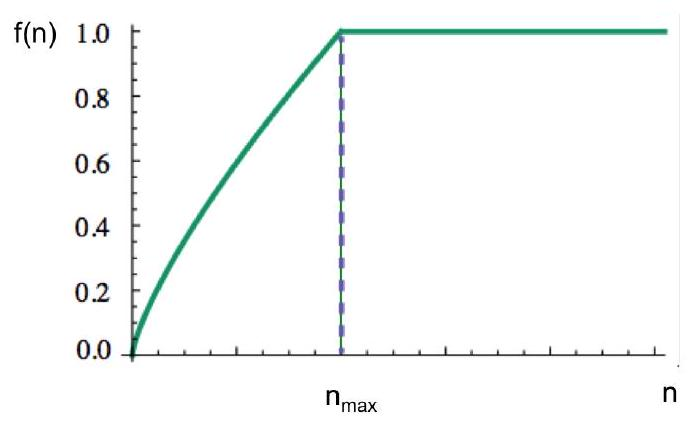
\includegraphics[max width=\textwidth]{2023_12_29_a68c38042b8470fb184bg-05}
\end{center}

\section*{Choosing $K$}
$K$ e.g. 50, 100, 500

\section*{Word Analogies}
\begin{center}
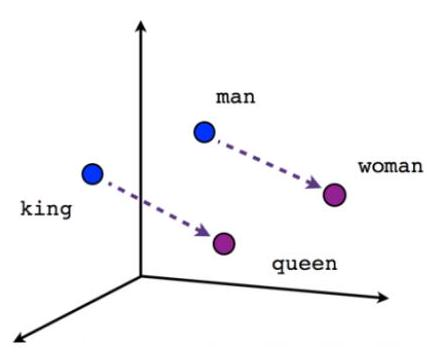
\includegraphics[max width=\textwidth]{2023_12_29_a68c38042b8470fb184bg-06(1)}
\end{center}

Male-Female

\begin{center}
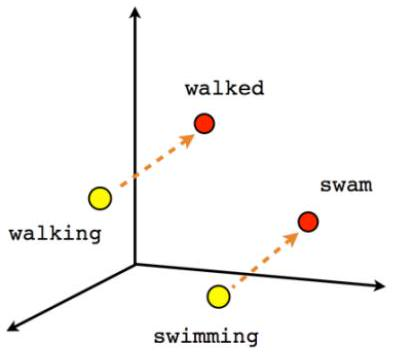
\includegraphics[max width=\textwidth]{2023_12_29_a68c38042b8470fb184bg-06(2)}
\end{center}

Verb tense

\begin{center}
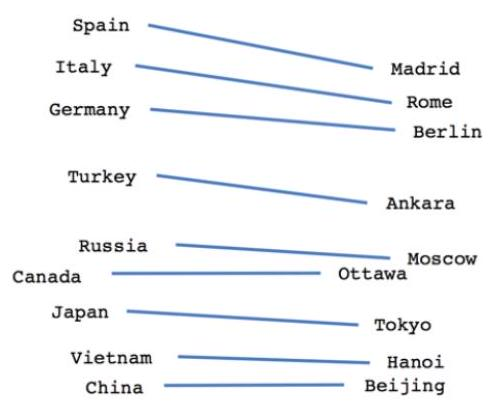
\includegraphics[max width=\textwidth]{2023_12_29_a68c38042b8470fb184bg-06}
\end{center}

Country-Capital

% \begin{center}
% \begin{tabular}{|cr||cc|}
% \hline
% \multicolumn{5}{|c|}{Newspapers} &  &  \\
% \hline
% \begin{tabular}{c}
% New York \\
% San Jose \\
% \end{tabular} & New York Times & Baltimore & Baltimore Sun &  &  &  \\
% San Jose Mercury News & Cincinnati & Cincinnati Enquirer &  &  &  &  \\
% \hline
% \multicolumn{5}{r|}{NHL Teams} &  &  \\
% \hline
% Boston & Boston Bruins & Montreal & Montreal Canadiens &  &  &  \\
% Phoenix & Phoenix Coyotes & Nashville & Nashville Predators &  &  &  \\
% \hline
% Detroit & NBA Teams &  &  &  &  &  \\
% \hline
% Oakland & Detroit Pistons & Toronto & Toronto Raptors &  &  &  \\
% \hline
% \multicolumn{5}{c||}{Golden State Warriors} & Memphis & Memphis Grizzlies \\
% \hline
% Austria & Austrian Airlines & Spain &  &  &  &  \\
% \hline
% Belgium & Brussels Airlines & Greece & Aegean Airlines &  &  &  \\
% \hline
% Steve Ballmer & Company executives &  &  &  &  &  \\
% \hline
% Samuel J. Palmisano & Microsoft & Larry Page & Google &  &  &  \\
% \hline
% \end{tabular}
% \end{center}

\section*{Training}
\begin{itemize}
  \item Stochastic Gradient Descent (SGD)
  \item Alternating Least-Squares (ALS)
\end{itemize}

Open questions:

\begin{itemize}
  \item Parallel and distributed training
  \item Does regularization help?
\end{itemize}

\section*{Alternative: Skip-Gram Model}
(Original word2vec)

Uses binary classification (logistic regression objective), to separate real word pairs $\left(w_{d}, w_{n}\right)$ from fake word pairs. Same inner product score $=$ matrix factorization.

Given $w_{d}$, a context word $w_{n}$ is

\begin{itemize}
  \item real $=$ appearing together in a context window of size 5
  \item fake $=$ any word $w_{n^{\prime}}$ sampled randomly: Negative sampling (also: Noise Contrastive Estimation)
\end{itemize}

\section*{Learning Representations of Sentences \& Documents}
Supervised: For a supervised task (e.g. predicting the emotion of a tweet), we can use matrixfactorization (below) or convolutional neural networks (see next weeks).

\begin{center}
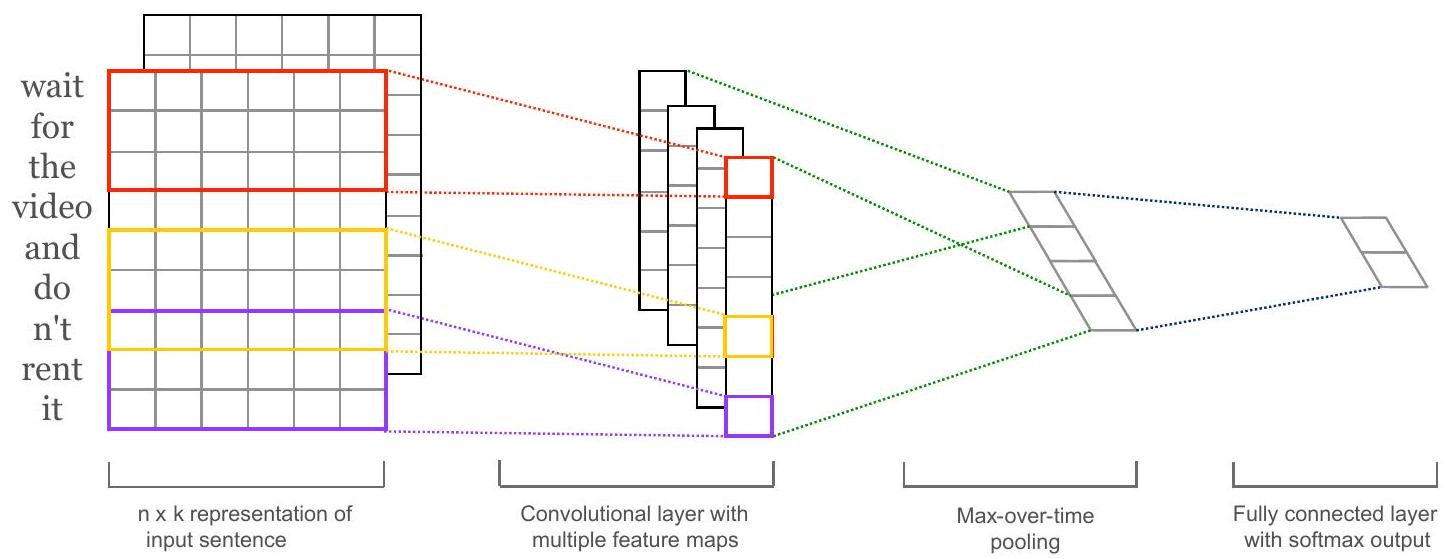
\includegraphics[max width=\textwidth]{2023_12_29_a68c38042b8470fb184bg-08}
\end{center}

$\rightarrow$ SemEval competition for tweet classification.

\section*{Unsupervised:}
\begin{itemize}
  \item Adding or averaging (fixed, given) word vectors
  \item Training word vectors such that adding/averaging works well
  \item Direct unsupervised training for sentences (appearing together with context sentences) instead of words
\end{itemize}

\section*{Fast Text}
Matrix factorization to learn document/sentence representations (supervised).

Given a sentence $s_{n}=$ $\left(w_{1}, w_{2}, \ldots, w_{m}\right)$, let $\mathbf{x}_{n} \in \mathbb{R}^{|\mathcal{V}|}$ be the bag-of-words representation of the sentence.

$$
\min _{\mathbf{W}, \mathbf{Z}} \mathcal{L}(\mathbf{W}, \mathbf{Z}):=\sum_{s_{n} \text { a sentence }} f\left(y_{n} \mathbf{W} \mathbf{Z}^{\top} \mathbf{x}_{n}\right)
$$

where $\mathbf{W} \in \mathbb{R}^{1 \times K}, \mathbf{Z} \in \mathbb{R}^{|\mathcal{V}| \times K}$ are the variables, and the vector $\mathbf{x}_{n} \in \mathbb{R}^{|\mathcal{V}|}$ represents our $n$-th training sentence.

Here $f$ is a linear classifier loss function, and $y_{n} \in\{ \pm 1\}$ is the classification label for sentence $\mathbf{x}_{n}$.

\section*{Language Models}
\section*{Selfsupervised training:}
Can a model generate text? - train classifier to predict the continuation (next word) of given text

\begin{itemize}
  \item Multi-class:
\end{itemize}

Use soft-max loss function with a large number of classes $D=$ vocabulary size

\begin{itemize}
  \item Binary classification:
\end{itemize}

Predict if next word is real or fake (i.e. as in word2vec)

Impressive recent progress using large models, such as transformers

(e.g. GPT-2, GPT-3, chatGPT

\href{https://transformer}{https://transformer} \href{http://huggingface.co/doc/gpt2-large}{huggingface.co/doc/gpt2-large},

\href{https://chat.openai.com/}{https://chat.openai.com/})

Arithmetic:

\begin{center}
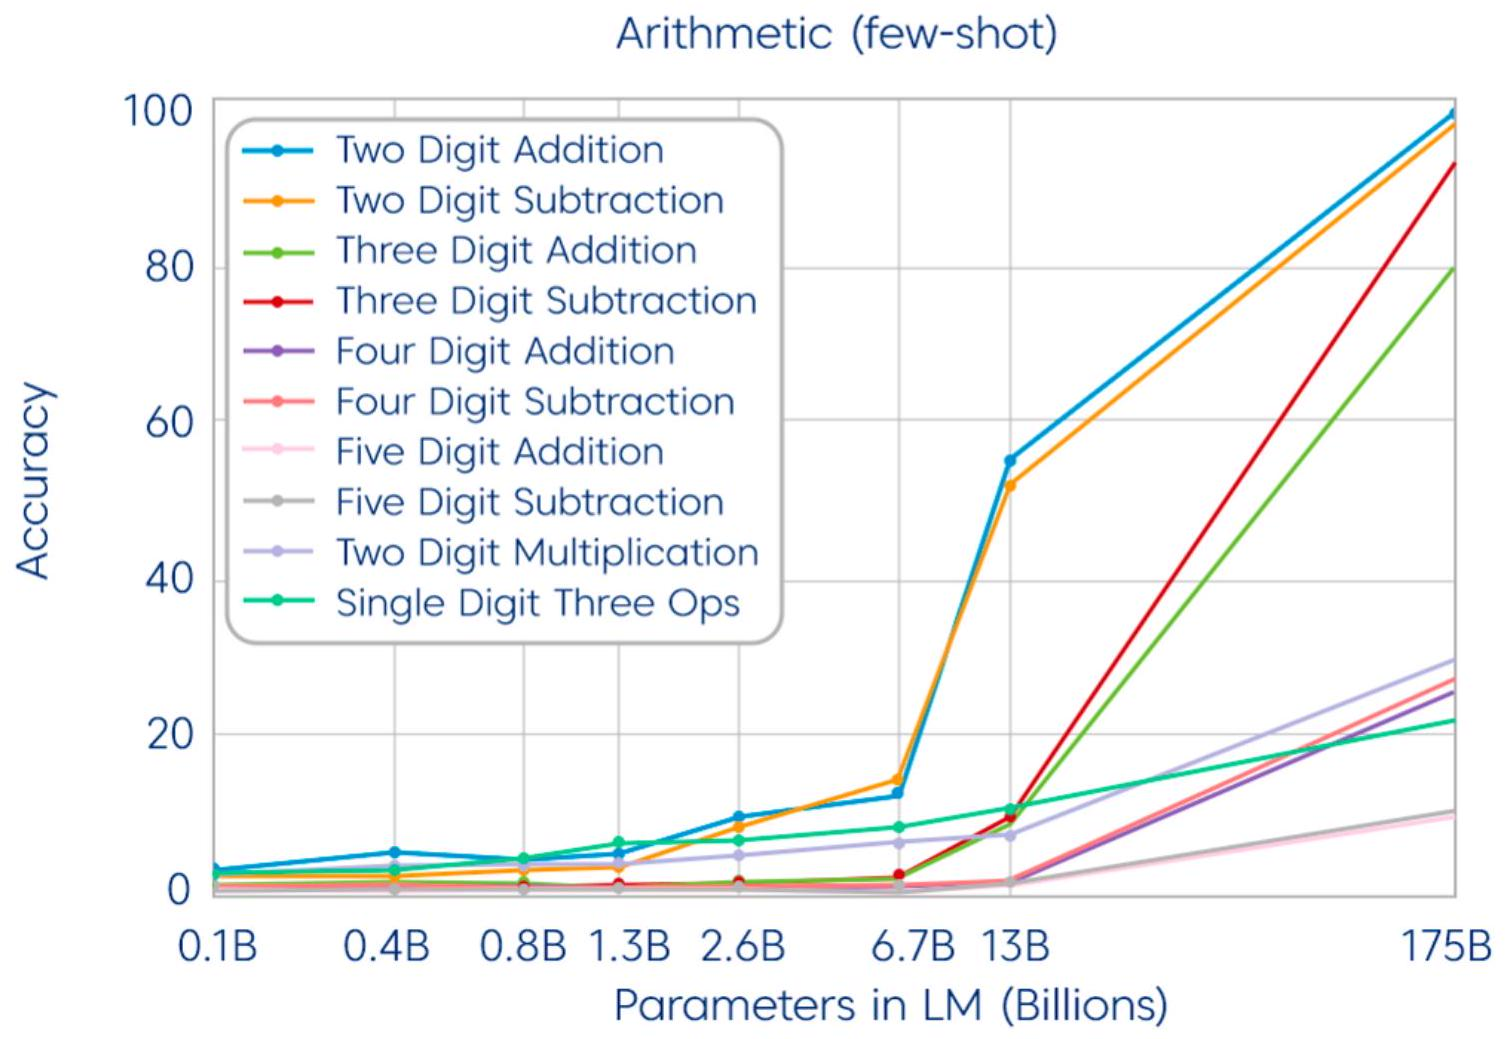
\includegraphics[max width=\textwidth]{2023_12_29_a68c38042b8470fb184bg-11}
\end{center}

Reasoning:

Maksym Andriushchenko @maksym\_andr

I got curious about this and tested ChatGPT on last year's exam from our ML course at EPFL

(\href{http://github.com/epfml/ML_course}{github.com/epfml/ML\_course}). Chain-of-thought evaluation with a majority vote over 5 trials gives 10/20

link: chatGPT on ML course exam

\section*{Further Pointers}
\begin{enumerate}
  \item word2vec:
\end{enumerate}

code: \href{http://code.google.com/p/word2vec/}{code.google.com/p/word2vec/}

paper:

"Distributed representations of words and phrases and their compositionality" - T Mikolov, I Sutskever, K Chen, GS Corrado, J Dean. NIPS 2013

\begin{enumerate}
  \setcounter{enumi}{1}
  \item GloVe:
\end{enumerate}

code and vectors: \href{http://nlp.stanford.edu/projects/glove/}{nlp.stanford.edu/projects/glove/}

paper:

"GloVe: Global Vectors for Word Representation" - Pennington, J., Socher, R., Manning, C. D.. EMNLP 2014

\begin{enumerate}
  \setcounter{enumi}{2}
  \item FastText \& sent2vec
\end{enumerate}

code: \href{http://github.com/facebookresearch/fastText}{github.com/facebookresearch/fastText}

papers:

"Bag of Tricks for Efficient Text Classification" - Joulin, A., Grave, E., Bojanowski, P., Mikolov, T. - EC-ACL, 2017.

"Enriching Word Vectors with Subword Information" - Bojanowski,

P., Grave, E., Joulin, A., Mikolov, T. - TACL, 2017.

"Unsupervised Learning of Sentence Embeddings using Compositional n-Gram Features" - Pagliardini, M., Gupta, P., Jaggi, M. NAACL 2018.

\begin{enumerate}
  \setcounter{enumi}{3}
  \item Write with transformers:
\end{enumerate}

code and demo: \href{http://transformer.huggingface.co/doc/gpt2-large}{transformer.huggingface.co/doc/gpt2-large}

\begin{enumerate}
  \setcounter{enumi}{4}
  \item ChatGPT
\end{enumerate}

demo: \href{http://chat.openai.com/}{chat.openai.com/}


\end{document}